\section{Additional experiments and details}
\label{app:experiments}

% In the following, we follow the convention where the $\ell$\textsuperscript{th} preactivation evaluated at input $x_\alpha$ is defined as
% \begin{equation}
%   z_{i, \alpha}^{(\ell)} = \sum_{i=1}^{n_\ell} W_{ij}^{(\ell)} \sigma(z_{j, \alpha}^{(\ell-1)}) + b_i^{(\ell)} \,,
%   \label{eq:preactivation_definition}
% \end{equation}

\subsection{Stability analysis}

In this section we provide additional experiments verifying the simultaneous stability of the NNGP $K$, the four-point cumulant $V_4$ as well as the four tensors $A, B, D$ and $F$ with increasing network depth $\ell$. Furthermore, we provide details of the numerical setup.

All experiments in this section are performed on a ReLU MLP without biases.
For the inputs, each component of all  vectors was drawn from a standard normal distribution. For the tensors $A, B, D$ and $F$ we thus used
\begin{align}
  x_0 &= ( -0.9895229339599609, -0.5992491841316223), \label{eq:x0_input} \\
  x_1 &= (-0.17877478897571564, 2.253682851791382), \label{eq:x1_input} \\
  x_2 &= (1.0237634181976318, -0.4618060886859894), \label{eq:x2_input} \\
  x_3 &= (-0.5364212393760681, 1.9298086166381836) \label{eq:x3_input}.
\end{align}
For the two-dimensional tensors $K$ and $\Theta$, only $x_0$ and $x_1$ were used. For the $V_4$ computation, we used 4-dimensional inputs resulting in
\begin{alignat}{4}
  &x_0 = ( && -0.9895229339599609, && -0.5992491841316223, \nonumber \\
  & && -0.17877478897571564, && +2.253682851791382), \\
  &x_1 = (&& +1.0237634181976318, && -0.4618060886859894, \nonumber \\
  & && -0.5364212393760681, && +1.9298086166381836), \\
  &x_2 = (&& -1.95197594165802, && -1.7220025062561035, \nonumber \\
  & && +0.8821542859077454, && -1.1963286399841309), \\
  &x_3 = (&& -0.1944112777709961, && -0.540934145450592, \nonumber \\ 
  & && +0.3308846354484558, && +0.0907512903213501).
\end{alignat}

% Further details are given in the corresponding results.

\textbf{Monte--Carlo estimation of the kernels.} The mean NTK and the mean NNGP are estimated by averaging over $N_\text{net}$ initializations of the network, i.e.\
\begin{align}
  \overline{K}^{(\ell)}_{\alpha \beta} &= \frac{1}{N_\text{net}} \sum_{I=1}^{N_\text{net}} z^{(\ell)}_{I;i,\alpha} z^{(\ell)}_{I;i,\beta} \,, \label{eq:nngp_mc}\\
\overline{\Theta}^{(\ell)}_{\alpha \beta} &= \frac{1}{N_\text{net}} \sum_{I=1}^{N_\text{net}} \left( \sum_{\mu}\frac{\partial z^{(\ell)}_{I;i,\alpha}}{\partial\theta_{\mu}}\frac{\partial z^{(\ell)}_{I; i, \beta}}{\partial\theta_{\mu}}\right) \,,
\end{align}
where $i$ is an arbitrary but fixed channel in the corresponding layer and $I$ labels the different initializations. The error bars correspond to the standard deviation of the mean and are estimated by dividing the sample standard deviation of the individual samples by $\sqrt{N_\text{net}}$. Due to the symmetries
\begin{equation}
  V^{(\ell)}_{\alpha \beta \gamma \delta} = V^{(\ell)}_{\beta \alpha \gamma \delta} = V^{(\ell)}_{\alpha \beta \delta \gamma} = V^{(\ell)}_{\gamma \delta \alpha \beta} \, ,
  \label{eq:v4_symmetries}
\end{equation}
there are 55 independent components of this tensor. We compute the same subset as presented in \cite{banta2024}.


\textbf{Linear scaling of the NTK $\Theta$ at criticality.} The purple line in Figure \ref{fig:ntk_comparison} (middle) shows the predicted linear scaling of the single-input NTK component for scale-invariant activation functions when setting $C_W^{(\ell)} = C_W^\mathrm{c}$ \cite{roberts2022}. For a bias-free ReLU MLP, it is given by
\begin{equation}
  \Theta^{(\ell)}_{\alpha \alpha} = \frac{1}{n_0} \|x_\alpha\|^2  \ell \,.
\end{equation}

\begin{figure}
    \begin{center}
        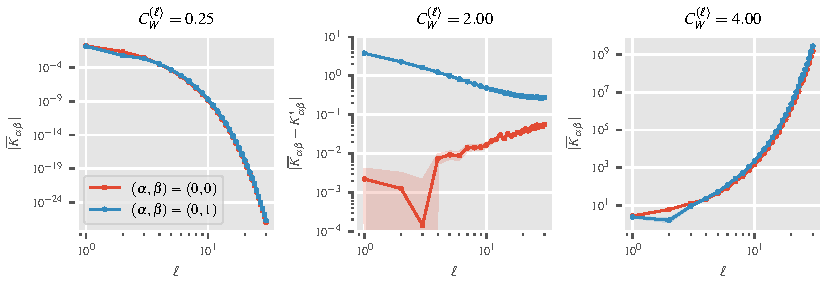
\includegraphics[width=0.99\textwidth]{figures/experiments/nngp_comparison.pdf}
    \end{center}
    \caption{\emph{Variance stability.} Components of the Monte--Carlo estimated NNGP $\overline{K}_{\alpha \beta}$ of a ReLU MLP as a function of layer depth $\ell$ corresponding to single and dinstinct inputs are shown for three different choices of $C_W^{(\ell)}$. The hidden layers are of size \num{200}. The middle plot shows the deviation of the NNGP component to the predicted fixed point kernel $K^*_{\alpha \beta}$ at the critical value $C_W^{(\ell)} = C_{W}^\mathrm{c} = 2$ (see text). Sample means are obtained from \num{1000} initializations for the non-critical cases (left and right), whereas the result in the middle is obtained from a sample size of $N_\text{net} = \num{e6}$. Error bars are included in all three plots (see text).}\label{fig:nngp_comparison}
\end{figure}
\textbf{Variance stability.} For completeness, in Figure \ref{fig:nngp_comparison} we show the stability analysis of the variance corresponding to the same setup that was used for the gradient analysis shown in Figure \ref{fig:ntk_comparison}, verifying the simultaneous stability of the NNGP and the NTK at the critical value $C_W^\mathrm{c}$. Note that the variance has already been studied numerically in \cite{banta2024}. As argued in \cite{roberts2022,halverson2021,banta2024}, there exists a non-trivial fixed point kernel $K^*_{\alpha \beta} \notin \{0, \infty\}$ for a ReLU MLP at criticality. It is given by
\begin{equation}
  K^*_{\alpha \beta} = \frac{C_W^\mathrm{c}}{n_0} \|x_\alpha\| \|x_\beta\| \, ,
  \label{eq:fixed_point_kernel_relu}
\end{equation}
where $n_0$ denotes the dimension of the input space, and is subtracted from the estimated NNGP in Figure \ref{fig:nngp_comparison} (middle).

\textbf{Monte--Carlo estimation of the four-point cumulant $V_4$.} Using \eqref{eq:nngp_mc}, we estimate the four-point cumulant $V_4$ to first order by
\begin{equation}
  \overline{V}^{(\ell)}_{\alpha \beta \gamma \delta} = \left(\frac{1}{N_\text{net}} \sum_{I=1}^{N_\text{net}} \frac{n_{\ell -1}}{n_{\ell} (n_{\ell}-1)} \sum_{\substack{i, j = 1 \\i \ne j}}^{n_\ell} z^{(\ell)}_{I;i,\alpha} z^{(\ell)}_{I;i,\beta} z^{(\ell)}_{I;j,\gamma} z^{(\ell)}_{I;j,\delta}\right)  - n_{\ell-1}\overline{K}^{(\ell)}_{\alpha \beta} \overline{K}^{(\ell)}_{\gamma \delta}+ \mathcal{O}\left(\frac{1}{n}\right) \,.
\end{equation}
In contrast to \eqref{eq:nngp_mc}, we exploit the fact here that all diagonal elements agree in expectation, i.e. we compute
\begin{equation}
  \overline{K}^{(\ell)}_{\alpha \beta} = \frac{1}{N_\text{net}} \sum_{I=1}^{N_\text{net}} \frac{1}{n_\ell} \sum_{i=1}^{n_{\ell}}z^{(\ell)}_{I;i,\alpha} z^{(\ell)}_{I;i,\beta} \, .\label{eq:nngp_trace_avg}
\end{equation}

In order to obtain statistics of this estimate, we repeat the Monte--Carlo sampling $N_\text{stats}$ times (for both $V_4$ and $K$) and take the corresponding mean and standard deviation as the estimate for $V_4$ and its error, respectively. The results for up to $\ell = 30$ are shown in Figure \ref{fig:v4_comparison_critical} for the critical case and in Figure \ref{fig:v4_comparison_non_critical} for the non-critical case. In addition to the result in \cite{banta2024}, we also provide regressions of the asymptotic power laws in the critical case, confirming the stability of $V_{4}$.

\textbf{Monte--Carlo estimation of the tensors $A, B, D$ and $F$.} Similarly to $V_4$, the tensors are estimated to first order by
\begin{align}
  \overline{A}^{(\ell)}_{\alpha\beta\gamma\delta} &= \frac{1}{N_\text{net}}\sum_{I=1}^{N_\text{net}}\frac{n_{\ell-1}}{n_{\ell}^2}\sum_{i,j=1}^{n_{\ell}}\widehat{\Delta\Theta}^{(\ell)}_{I;ii,\alpha\beta}\widehat{\Delta \Theta}_{I;jj,\gamma\delta}^{(\ell)} + \mathcal{O}\left(\frac{1}{n}\right) \\
  \overline{B}^{(\ell)}_{\alpha\gamma\beta\delta} &= \frac{1}{N_\text{net}}\sum_{I=1}^{N_\text{net}}\frac{n_{\ell-1}}{n_{\ell}^2}\sum_{i,j=1}^{n_{\ell}}\widehat{\Delta\Theta}^{(\ell)}_{I;ij,\alpha\beta}\widehat{\Delta \Theta}_{I;ij,\gamma\delta}^{(\ell)} + \mathcal{O}\left(\frac{1}{n}\right) \\
  \overline{D}^{(\ell)}_{\alpha\beta\gamma\delta} &= \frac{1}{N_\text{net}}\sum_{I=1}^{N_\text{net}}\frac{n_{\ell-1}}{n_{\ell}^2}\sum_{i,j=1}^{n_{\ell}}z_{I;i,\alpha}^{(\ell)}z_{I;i,\beta}^{(\ell)}\widehat{\Delta \Theta}_{I;jj,\gamma\delta}^{(\ell)} + \mathcal{O}\left(\frac{1}{n}\right) \\
  \overline{F}^{(\ell)}_{\alpha\gamma\beta\delta} &= \frac{1}{N_\text{net}}\sum_{I=1}^{N_\text{net}}\frac{n_{\ell-1}}{n_{\ell}^2}\sum_{i,j=1}^{n_{\ell}}z_{I;i,\alpha}^{(\ell)}z_{I;j,\beta}^{(\ell)}\widehat{\Delta \Theta}_{I;ij,\gamma\delta}^{(\ell)} + \mathcal{O}\left(\frac{1}{n}\right) \, ,
\end{align}
where the NTK fluctuation $\widehat{\Delta \Theta}^{(\ell)}_{ij,\alpha \beta}$was already introduced in Section \ref{sec-finitewidth-corrections-NTK}. Again, the computation is repeated $N_\text{stats}$ times to obtain the mean and standard deviation of the estimate. For each of these tensors, the critical and non-critical cases are computed for the same input combinations as for $V_4$ up to $\ell =30$. The results for tensor $A$ are shown in Figures \ref{fig:A_comparison_critical} \& \ref{fig:A_comparison_non_critical}, for tensor $B$ in Figures \ref{fig:B_comparison_critical} \& \ref{fig:B_comparison_non_critical}, for tensor $D$ in Figures \ref{fig:D_comparison_critical} \& \ref{fig:D_comparison_non_critical} and for tensor $F$ in Figures \ref{fig:F_comparison_critical} \& \ref{fig:F_comparison_non_critical}. The regression of the asymptotic power laws is shown in blue for the critical cases. The power-law behavior at criticality for all tested components confirms that the NTK-tensors $A$, $B$, $D$ and $F$ are also stabilized by the critical initialization variance of the infinite width limit.

\begin{figure}
    \begin{center}
        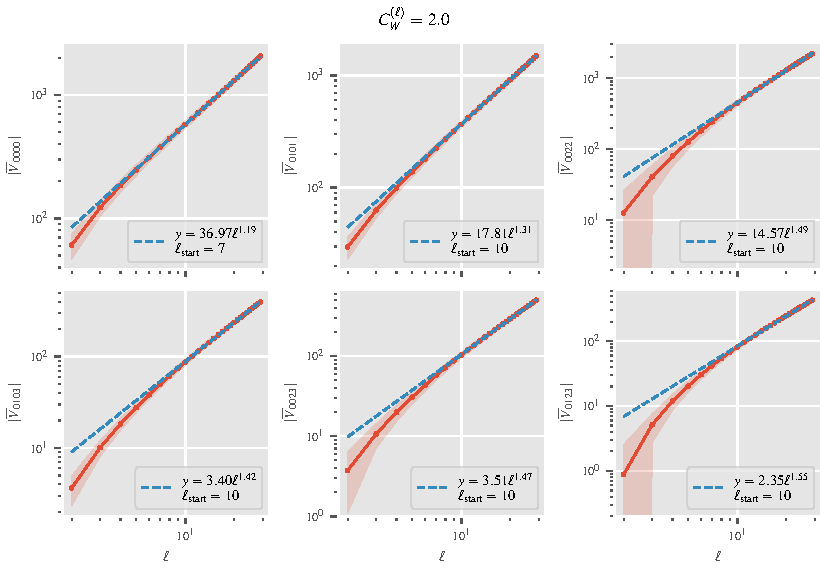
\includegraphics[width=0.99\textwidth]{figures/experiments/v4_comparison_critical.pdf}
    \end{center}
    \caption{\emph{Stability of the four-point cumulant $V_4$ at criticality.} Selected components of the Monte--Carlo estimated tensor $\overline{V}_4$ of a ReLU MLP as a function of layer depth $\ell$ are shown for the critical value $C_W^{(\ell)} = C_W^\mathrm{c} = 2$. The hidden layers are of size \num{300}. A regression of the asymptotic power law is shown in blue. The lowest layer included in the regression is given by $\ell_\text{start}$. $\overline{V}_4$ is computed from $N_\text{net} = \num{e4}$ initializations and its mean and error bars are estimated from $N_\text{stats} = \num{1000}$ repetitions (see text).}\label{fig:v4_comparison_critical}
\end{figure}

\begin{figure}
  \begin{center}
    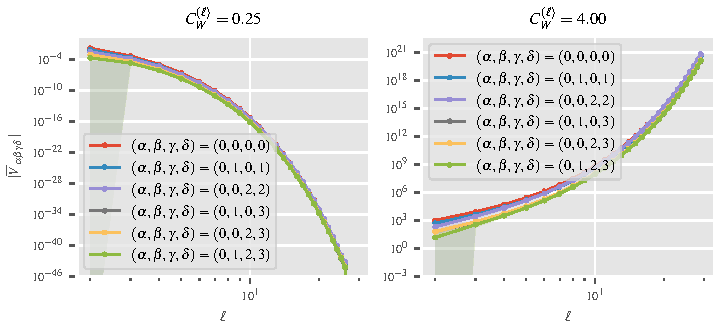
\includegraphics[width=0.95\textwidth]{figures/experiments/v4_comparison_non_critical.pdf}
  \end{center}
\caption{\emph{Instability of the four-point cumulant $V_4$ away from criticality.} Selected components of the Monte--Carlo estimated tensor $\overline{V}_4$ are shown for $C_W^{(\ell} < C_W^\mathrm{c}$ (left) and $C_W^{(\ell} > C_W^\mathrm{c}$ (right). $\overline{V}_4$ is computed from $N_\text{net} = \num{e4}$ initializations and its mean and error bars are estimated from  $N_\text{stats} = \num{1000}$ repetitions (see text).}\label{fig:v4_comparison_non_critical}
\end{figure}

\begin{figure}
    \begin{center}
        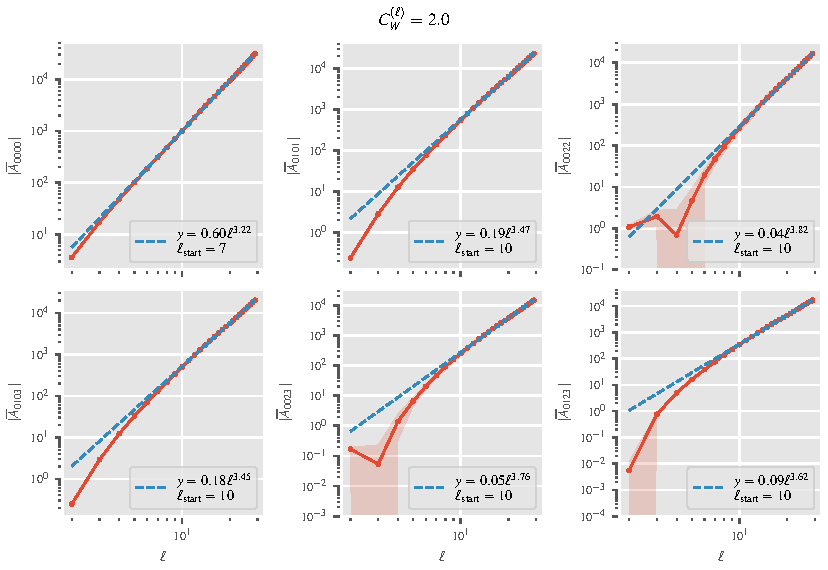
\includegraphics[width=0.99\textwidth]{figures/experiments/A_comparison_critical.pdf}
    \end{center}
    \caption{\emph{Stability of the $A$ tensor at criticality.} Selected components of the Monte--Carlo estimated tensor $\overline{A}$ of a ReLU MLP as a function of layer depth $\ell$ are shown for the critical value $C_W^{(\ell)} = C_W^\mathrm{c} = 2$. The hidden layers are of size \num{200}. A regression of the asymptotic power law is shown in blue. The lowest layer included in the regression is given by $\ell_\text{start}$. $\overline{A}$ is computed from $N_\text{net} = \num{600}$ initializations and its mean and error bars are estimated from $N_\text{stats} = \num{10}$ repetitions (see text).}\label{fig:A_comparison_critical}
\end{figure}

\begin{figure}
  \begin{center}
    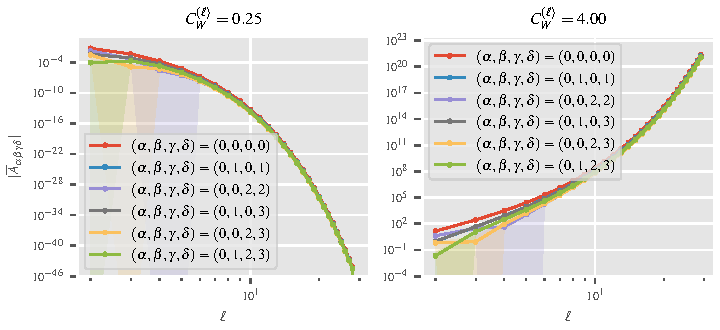
\includegraphics[width=0.95\textwidth]{figures/experiments/A_comparison_non_critical.pdf}
  \end{center}
  \caption{\emph{Instability of the $A$ tensor away from criticality.} Selected components of the Monte--Carlo estimated tensor $\overline{A}$ are shown for $C_W^{(\ell} < C_W^\mathrm{c}$ (left) and $C_W^{(\ell} > C_W^\mathrm{c}$ (right). $\overline{A}$ is computed from $N_\text{net} = \num{600}$ initializations and its mean and error bars are estimated from  $N_\text{stats} = \num{10}$ repetitions (see text).}\label{fig:A_comparison_non_critical}
\end{figure}

\begin{figure}
    \begin{center}
        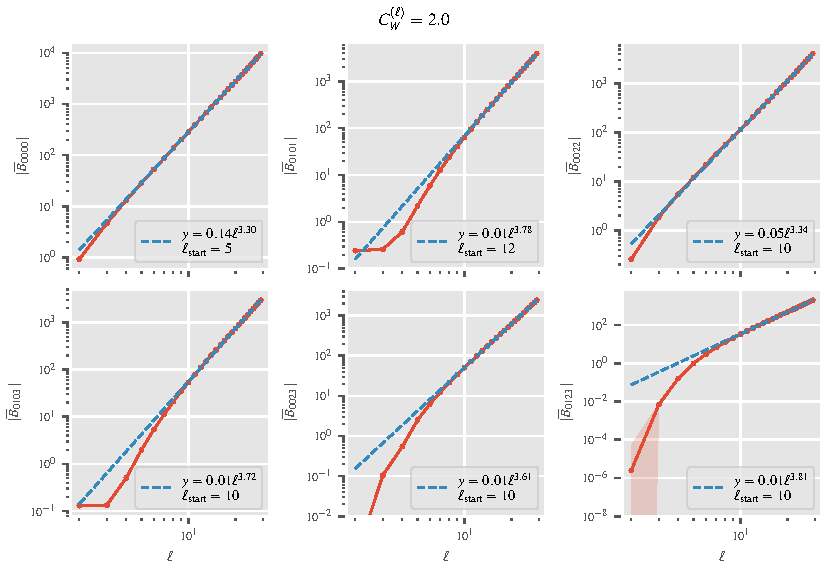
\includegraphics[width=0.99\textwidth]{figures/experiments/B_comparison_critical.pdf}
    \end{center}
    \caption{\emph{Stability of the $B$ tensor at criticality.} Selected components of the Monte--Carlo estimated tensor $\overline{B}$ of a ReLU MLP as a function of layer depth $\ell$ are shown for the critical value $C_W^{(\ell)} = C_W^\mathrm{c} = 2$. The hidden layers are of size \num{200}. A regression of the asymptotic power law is shown in blue. The lowest layer included in the regression is given by $\ell_\text{start}$. $\overline{B}$ is computed from $N_\text{net} = \num{600}$ initializations and its mean and error bars are estimated from $N_\text{stats} = \num{10}$ repetitions (see text).}\label{fig:B_comparison_critical}
\end{figure}

\begin{figure}
  \begin{center}
    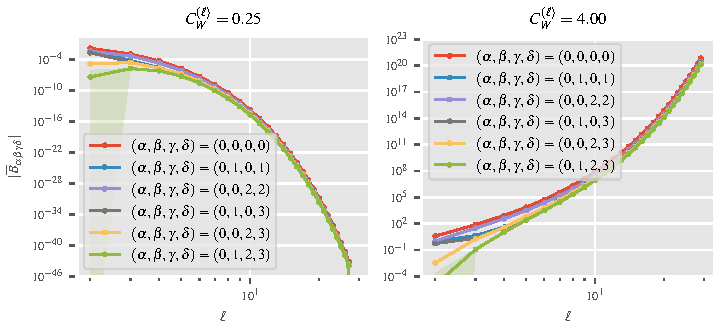
\includegraphics[width=0.95\textwidth]{figures/experiments/B_comparison_non_critical.pdf}
  \end{center}
  \caption{\emph{Instability of the $B$ tensor away from criticality.} Selected components of the Monte--Carlo estimated tensor $\overline{B}$ are shown for $C_W^{(\ell} < C_W^\mathrm{c}$ (left) and $C_W^{(\ell} > C_W^\mathrm{c}$ (right). $\overline{B}$ is computed from $N_\text{net} = \num{600}$ initializations and its mean and error bars are estimated from  $N_\text{stats} = \num{10}$ repetitions (see text).}\label{fig:B_comparison_non_critical}
\end{figure}

\begin{figure}
    \begin{center}
        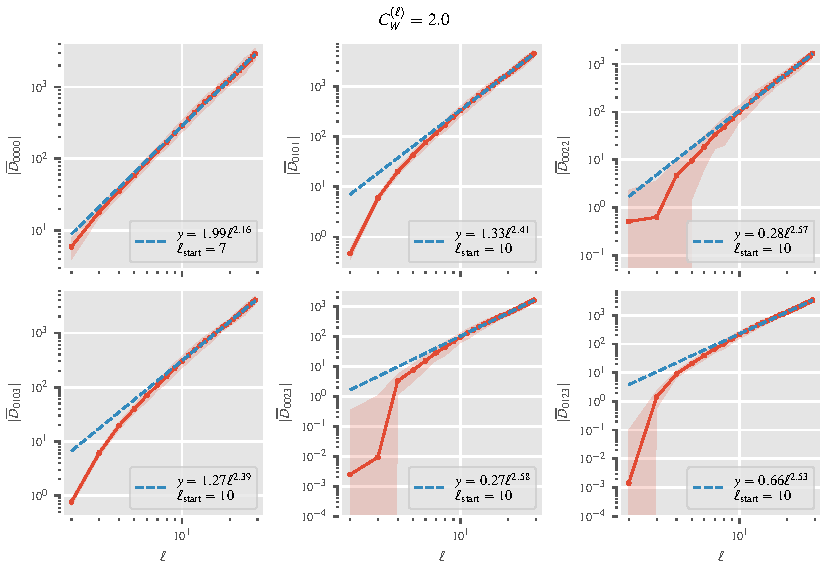
\includegraphics[width=0.99\textwidth]{figures/experiments/D_comparison_critical.pdf}
    \end{center}
    \caption{\emph{Stability of the $D$ tensor at criticality.} Selected components of the Monte--Carlo estimated tensor $\overline{D}$ of a ReLU MLP as a function of layer depth $\ell$ are shown for the critical value $C_W^{(\ell)} = C_W^\mathrm{c} = 2$. The hidden layers are of size \num{200}. A regression of the asymptotic power law is shown in blue. The lowest layer included in the regression is given by $\ell_\text{start}$. $\overline{D}$ is computed from $N_\text{net} = \num{600}$ initializations and its mean and error bars are estimated from $N_\text{stats} = \num{10}$ repetitions (see text).}\label{fig:D_comparison_critical}
\end{figure}

\begin{figure}
  \begin{center}
    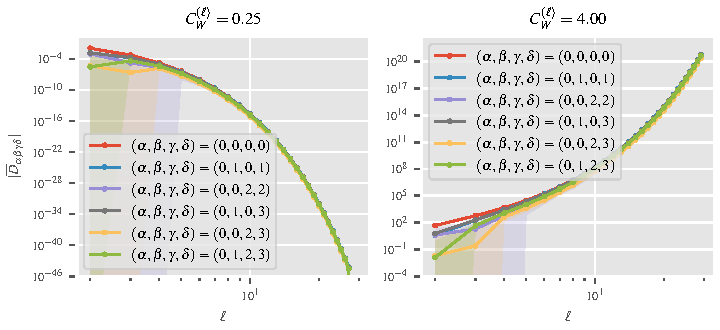
\includegraphics[width=0.95\textwidth]{figures/experiments/D_comparison_non_critical.pdf}
  \end{center}
  \caption{\emph{Instability of the $D$ tensor away from criticality.} Selected components of the Monte--Carlo estimated tensor $\overline{D}$ are shown for $C_W^{(\ell} < C_W^\mathrm{c}$ (left) and $C_W^{(\ell} > C_W^\mathrm{c}$ (right). $\overline{D}$ is computed from $N_\text{net} = \num{600}$ initializations and its mean and error bars are estimated from  $N_\text{stats} = \num{10}$ repetitions (see text).}\label{fig:D_comparison_non_critical}
\end{figure}

\begin{figure}
    \begin{center}
        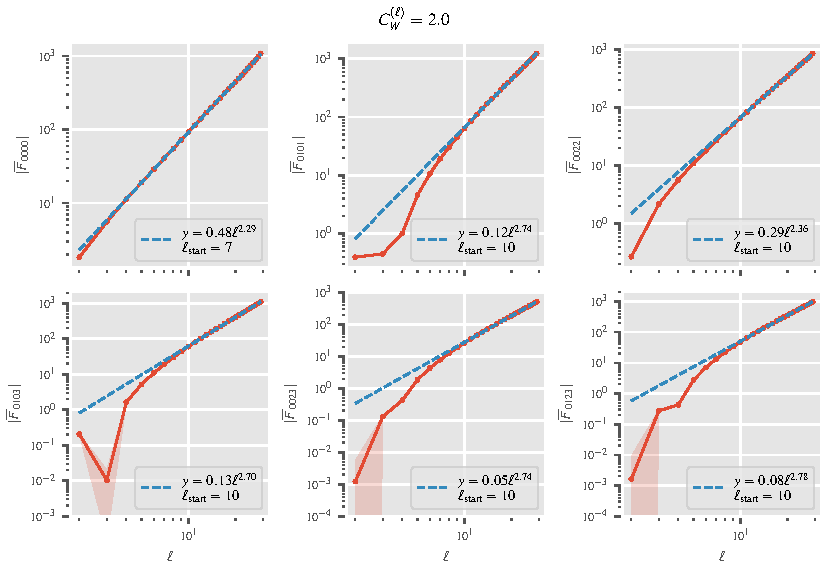
\includegraphics[width=0.99\textwidth]{figures/experiments/F_comparison_critical.pdf}
    \end{center}
    \caption{\emph{Stability of the $F$ tensor at criticality.} Selected components of the Monte--Carlo estimated tensor $\overline{F}$ of a ReLU MLP as a function of layer depth $\ell$ are shown for the critical value $C_W^{(\ell)} = C_W^\mathrm{c} = 2$. The hidden layers are of size \num{200}. A regression of the asymptotic power law is shown in blue. The lowest layer included in the regression is given by $\ell_\text{start}$. $\overline{F}$ is computed from $N_\text{net} = \num{600}$ initializations and its mean and error bars are estimated from $N_\text{stats} = \num{10}$ repetitions (see text).}\label{fig:F_comparison_critical}
\end{figure}

\begin{figure}
  \begin{center}
    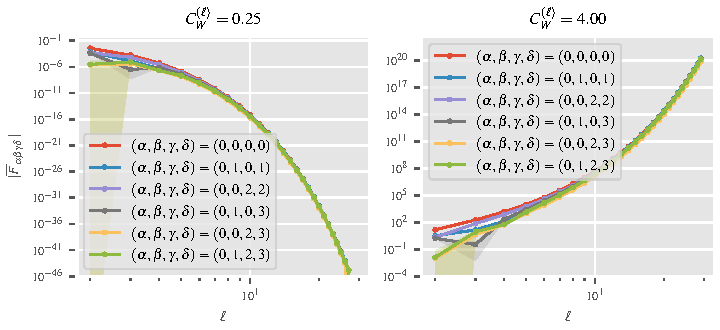
\includegraphics[width=0.95\textwidth]{figures/experiments/F_comparison_non_critical.pdf}
  \end{center}
  \caption{\emph{Instability of the $F$ tensor away from criticality.} Selected components of the Monte--Carlo estimated tensor $\overline{F}$ are shown for $C_W^{(\ell} < C_W^\mathrm{c}$ (left) and $C_W^{(\ell} > C_W^\mathrm{c}$ (right). $\overline{F}$ is computed from $N_\text{net} = \num{600}$ initializations and its mean and error bars are estimated from  $N_\text{stats} = \num{10}$ repetitions (see text).}\label{fig:F_comparison_non_critical}
\end{figure}


\subsection{Kernel-corrections for other scale-invariant and scale-dependent activation functions}

In the following we show the finite-width corrections for other activation functions than ReLU. We include two scale-invariant functions, namely the identity and the Leaky ReLU, and the scale-dependent GeLU activation to show the different qualitative behavior.
For all activations functions, we used again inputs $x_0$ and $x_1$ given in \eqref{eq:x0_input} \& \eqref{eq:x1_input}

\textbf{Estimating the finite-width corrections.} For a four-layer MLP without biases, we estimate the empirical NNGP according to \eqref{eq:nngp_trace_avg} and the NTK according to
\begin{equation}
  \overline{\Theta}^{(\ell)}_{\alpha \beta} = \frac{1}{N_\text{net}} \sum_{I=1}^{N_\text{net}} \left( \frac{1}{n_\ell} \sum_{i=1}^{n_\ell} \left( \sum_{\mu}\frac{\partial z^{(\ell)}_{I;i,\alpha}}{\partial\theta_{\mu}}\frac{\partial z^{(\ell)}_{I; i, \beta}}{\partial\theta_{\mu}}\right) \right) \,.
  \label{eq:ntk_trace_avg}
\end{equation}
The infinite-width solutions $K$ and $\Theta$ (assuming NTK parametrization) is computed with the \texttt{neural-tangents} \cite{novak2020a} library. Error estimates are obtained by dividing the sample variance of the estimated kernels by $\sqrt{N_\text{net}}$ and further rescaling them by $1/K$ or $1/\Theta$, respectively, since we are considering the relative deviations.

\textbf{The linear case.} Using the identity as the activation function, we obtain the result in Figure \ref{fig:identity_corrections}. Both the single- and distinct-input component do not show any corrections with width, as expected. The variance of the weights is $C_W^{(\ell)} = 2$.

\begin{figure}
  \begin{center}
    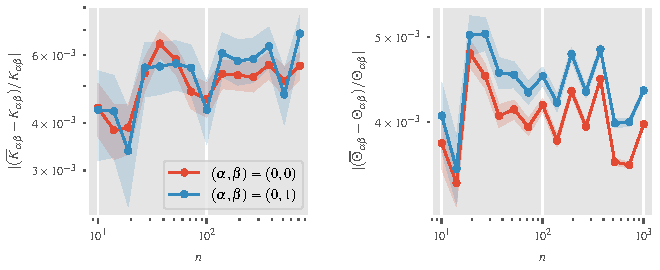
\includegraphics[width=0.95\textwidth]{figures/experiments/Identity_width_corrections_layer-4.pdf}
  \end{center}
  \caption{\emph{Finite-width corrections for the identity.} Relative deviations of the Monte--Carlo estimated NNGP and NTK to its infinite-width counterparts as a function of hidden layer width $n=n_\ell$. A four layer linear MLP with $C_W=2$ is sampled over $\num{5e6}$ initializations. Error bars of the sample mean are included for all lines. Both a single and distinct input component of each kernel is shown.}\label{fig:identity_corrections}
\end{figure}

\textbf{The Leaky ReLU case.} Using
\begin{equation}
  \sigma(x) = \alpha \, \mathrm{min}(x, 0) + \mathrm{max}(x, 0) \, ,  \label{eq:leakyrelu}
\end{equation}
with $\alpha = 0.1$ as the activation function, we observe similar behavior as for the ReLU as can be seen in Figure \ref{fig:leakyrelu_corrections}. While the distinct-input component shows a convergence to the infinite-width limit, the single-input component is already exact at any finite width, as expected due to the scale-invariant nature. Again, $C_W^{(\ell)} = 2$.

\begin{figure}
  \begin{center}
    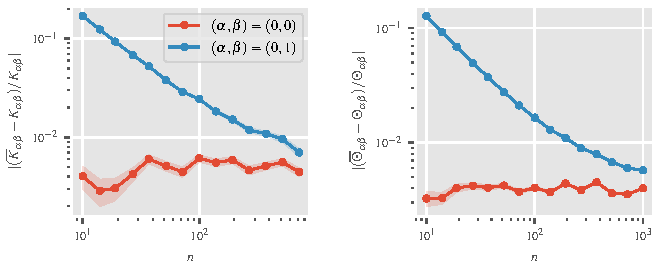
\includegraphics[width=0.95\textwidth]{figures/experiments/LeakyRelu_width_corrections_layer-4.pdf}
  \end{center}
  \caption{\emph{Finite-width corrections for Leaky ReLU.} Relative deviations of the Monte--Carlo estimated NNGP and NTK to its infinite-width counterparts as a function of hidden layer width $n=n_\ell$. A four layer Leaky ReLU MLP with $C_W=2$ is sampled over $\num{5e6}$ initializations. Error bars of the sample mean are included for all lines. Both a single and distinct input component of each kernel is shown.}\label{fig:leakyrelu_corrections}
\end{figure}

\textbf{The GeLU case.} To show the distinct behavior of scale-dependent activation functions, we repeat the same experiment for the GeLU function. As shown in Figure \ref{fig:gelu_corrections}, not only the distinct-input, but also the single-input component approach the infinite-width solution only with increasing width. Note that due to the scale-dependence, the scale of the input vectors affects the convergence behavior. Intuitively, large inputs emphasize the asymptotic regions of the activation function, rendering the corrections more similar to the ReLU case, whereas small inputs focus on the nearly linear region close to the origin, leading to a behavior similar to the linear case. Therefore, we rescaled the inputs $x_0$ and $x_1$ by a factor of \num{0.53} to make the distinct nature of this scale-dependent function more pronounced. The variance of the weights was set to $C_W^{(\ell)} = 1.98305826$ \cite{roberts2022}, in order to suppress significant change of magnitude of the preactivation values after a few layers.
\begin{figure}
  \begin{center}
    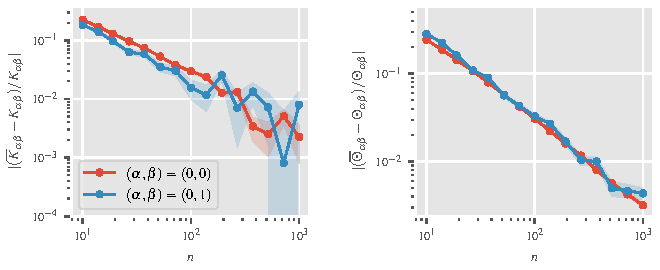
\includegraphics[width=0.95\textwidth]{figures/experiments/Gelu_width_corrections_layer-4_scale-0.53_double_prec.pdf}
  \end{center}
  \caption{\emph{Finite-width corrections for GeLU.} Relative deviations of the Monte--Carlo estimated NNGP and NTK to its infinite-width counterparts as a function of hidden layer width $n=n_\ell$. A four layer GeLU MLP with $C_W=2$ is sampled over $\num{5e5}$ initializations. Error bars of the sample mean are included for all lines. Both a single and distinct input component of each kernel is shown.}\label{fig:gelu_corrections}
\end{figure}

\subsection{Compute resources}

All presented experiments were conducted on a cluster equipped with NVIDIA A40 GPUs with 48GB of RAM. The stability analysis for the NNGP and $V_4$ could each be computed on a single GPU in less than two hours for all three values of $C_W$. Tensors involving the gradient are more expensive to compute, thus the layer width was reduced to \num{200}. On a single GPU, a single such tensor for three different values of $C_W$ was computed in less than 6 hours. Note that multiple tensors can be computed in parallel using the same ensemble.

Similarly, the finite-width corrections are fast to compute for the NNGP but more expensive for the NTK. For each activation function, it took less than three hours to obtain the results presented here.

%%% Local Variables:
%%% mode: LaTeX
%%% TeX-master: "ntk_feynman"
%%% End:
